

% real time models

%% cover basic RT scheduling
%%% EDF
%%% FP
%%% schedulability tests

% operating systems
%% resource kernels
%% microkernels

\chapter{Core concepts}
\label{chap:background}

In this section we provide the background required to motivate and understand our research.
We introduce real-time theory, including scheduling algorithms and resource sharing protocols.
In addition, we define operating systems, microkernels and introduce the concept of a resource kernel.
This thesis draws on all of these fields in order to support real-time and mixed-criticality systems.

\section{Real-time theory}
\label{sec:real-time-theory}

Real-time systems have timing constraints, where the correctness of the system is dependent not only
on the results of computations, but on the time at which those results arrive~\citep{Stankovic_88}.
Essentially all software is real-time: if the software never gets access to processing time, no
results will ever be obtained.  However, for a system to be considered real-time it must be
sensitive to timing behaviour---how much processing time is allocated and when it is allocated. For
most software, time is fungible: it does not matter when the software is run, as long as it does get
run. For real-time software this is not the case.  Consider the case of software that deploys the
brakes on a train: the routine must run in time for the train to stop at the platform. Or, in a more
critical scenario, software that deploys the landing gear on a plane: it must run and the gear must
be fully down before the plane hits the runway.

There are many ways to model real-time systems, which we touch on in the coming chapters. 

\subsection{Types of real-time tasks}

The term \emph{task} in real-time theory is used to refer to a single instruction stream, which in 
operating systems terms is referred to as a thread. How tasks
are realised by an operating system---with or without memory protection, for example---is specific to the
implementation.  Computations by tasks in real-time systems have deadlines which determine the
correctness of the system. How those deadlines effect correctness depends on the category of the
system, which is generally referred to as \gls{HRT}, \gls{SRT}, or \emph{best-effort}.

\emph{Hard Real-Time} tasks have absolute deadlines; if a deadline is missed,
the task is considered incorrect. \gls{HRT} tasks are most common in safety-critical systems, where
deadline misses lead to catastrophic results.  Examples include airbag systems
in cars and control systems for autonomous vehicles.  In the former, missing a deadline could cause
an airbag to be deployed too late.  In the latter, the autonomous vehicle could crash.  To guarantee
that a \gls{HRT} task can meet deadlines, the code must be subject to {\gls{WCET}} analysis. State
of the art {\gls{WCET}} analysis is generally pessimistic by several orders of magnitude, which
means that allocated time will not generally be used completely, although it must be available.
WCET is pessimistic for multiple reasons: firstly, much behaviour like interrupt arrival times, 
cannot be predicted but only
bounded, so the WCET includes the worst possible execution case. Secondly, accurate models of modern
hardware are few, so often the WCET must assume caches are not primed and possibly conflicting. 
Further detail about {\gls{WCET}} analysis can be found in \citet{Lv_GZDYZ_09}.

\emph{Soft Real-Time} tasks, as opposed to \gls{HRT}, can be
considered correct in the presence of some defined level of deadline misses. Although {\gls{WCET}}
can be known for {\gls{SRT}} tasks, less precise but more optimistic time estimates are generally
used for practicality.  Examples of \gls{SRT} tasks can be found in multimedia and video game platforms,
where deadline misses may result in some non-critical effect such as performance degradation.
\gls{SRT} tasks can also be found in safety-critical systems where the result degrades if not enough
time has been
allocated by the deadline, but the result remains useful \eg image recognition and object detection
in autonomous vehicles. In such tasks, a minimum allocation of time to the task might be \gls{HRT},
while further allocations are \gls{SRT}.

Various models exist to quantify permissible deadline misses in \gls{SRT} systems.  One measure is
to consider the upper bound of how much the deadline is missed, referred to as
\emph{tardiness}~\citep{Devi:phd}.  Another is to express an upper bound on the percentage of
deadline misses permitted for the system to be considered correct, which is easier to measure but
less meaningful. Some \gls{SRT} systems allow deadlines to be skipped
completely~\citep{Koren_Shasha_95} while others allow deadlines to be postponed. Systems that allow
deadlines to be skipped are often referred to as firm real-time \eg media processing, where some
frames can be dropped. 

\emph{best-effort} tasks do not have temporal requirements, and generally execute in the
background of a real-time system. Examples include logging services and standard applications, but
may be far more complicated. Of course, any task must be scheduled at some point for system success,
so there must be some timing guarantee. 

\subsection{Real-time models}

A real-time system is a collection of tasks, traditionally of the same model. If a system is
referred to as \gls{SRT}, then all tasks in that system are \gls{SRT}. For analysis, each task in a
real-time system is modelled as an infinite series of \emph{jobs}. Each job represents a computation
with a deadline. 
One practical model in common use is the \emph{sporadic task model}~\citep{Sprunt_SL_89a}, which can
model both \emph{periodic} and \emph{aperiodic} tasks and maps well onto typical control systems. 

\begin{listing}
    \begin{minted}{c}
for (;;) {
    // job arrives
    doJob();
    // job completes before deadline
    // sleep until next job is ready
    sleep();
}
    \end{minted}
\caption{Example of a basic sporadic real-time task.}
\label{list:sporadic}
\end{listing}


The sporadic task model considers a real-time system as a set of tasks, $A_{1},A_{2},\ldots,A_{n}$.
Each $A_{i}$ refers to a specific task in the task set, usually each for a different functionality.
The infinite series of jobs is per task, and represented by $A_{i1},A_{i2},\ldots,A{in}$. Each task has
a \gls{WCET}, $C_{i}$, and period, $T_{i}$, which represents the minimum inter-arrival time
between jobs. When a $T_{i}$ has passed and a job can run again, it is said to be \emph{released}.
When a job is ready to run, it is said to have \emph{arrived} and when a job finishes and blocks until
the next arrival, it is said to be \emph{completed}. 

For periodic tasks, which are commonly found in control systems, jobs release and arrive at the same
time; they are always ready to run once their period has passed. For aperiodic, \ie interrupt driven
tasks, the arrival time can be at or beyond the release time. 

\begin{table}[b]
\rowcolors{2}{gray!25}{white}
\centering
\begin{tabularx}{\textwidth}{cX}\toprule
    \emph{Notation} & \emph{Meaning} \\\midrule
    $A$               & A task set. \\
    $A_{i}$           & A specific task in a task set \\
    $A_{ij}$          & A specific job of a specific task set. \\
    $T_{i}$           & The minimum period of a task, the minimum time between job releases. \\
        $C_{i}$       & The \gls{WCET} of a task ($C_{i} \leq T_{i}$). \\
    $U_{i}$           & The maximum utilisation of task $i$, which is $\frac{C}{T}$ \\
    $D_{i}$           & The relative deadline of task $i$ \\
    $t_{ij}$          & The release time of the $j$th job of task $i$ \\
    $d_{ij}$          & The deadline for the $j$th job of task $i$. \\
    $a_{ij}$          & The arrival time of the $j$th job of task $i$, $a_{ij} \geq t_{ij}$ \\
    $n$               & The number of tasks in a task set\\
    \bottomrule
    \end{tabularx}
    \caption{Parameters and notation for the sporadic task model.}
    \label{t:notation}
\end{table}

Jobs must complete before their period has passed ($C_{i} \leq T_{i}$), as the model does not
support jobs that run simultaneously. Tasks with interleaving jobs must be modelled as separate
tasks which do not overlap.  \Cref{list:sporadic} shows pseudocode for a sporadic task and
\Cref{t:notation} summarises the notation which is used throughout this thesis.

Sporadic tasks have deadlines relative to their arrival time, which may be \emph{constrained} or
\emph{implicit}.  An \emph{implicit} deadline means the job must finish before the period elapses.
\emph{Constrained} deadlines are relative to the release time, but before the period elapses.  Other
task models allow for \emph{arbitrary} deadlines, which can be after the period elapses, however
arbitrary deadlines are not compatible with the sporadic task model without adjustment, as they allow multiple jobs from
one task to be active at one time.  In order to model tasks with arbitrary deadlines with the
sporadic task model, they must be split 
into multiple, different tasks with larger periods and
constrained deadlines.

\begin{figure}[t]
	\begin{center}
		\leavevmode
		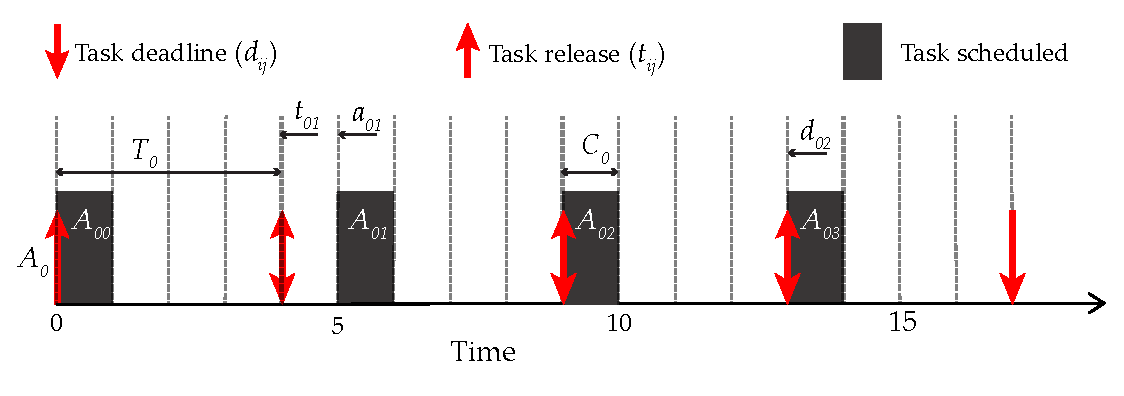
\includegraphics[width=\textwidth]{sporadic}
        \caption[Diagram of the sporadic task model.]{Diagram of the sporadic task model notation described in \cref{t:notation}, showing
        a task set $A$ with a single task $A_{0}$ where $T_{0} = 4$ and $C_{0} = 1$.}
		\label{fig:fp-schedule}
	\end{center}
\end{figure}


\section{Scheduling}
\label{sec:rt-scheduling}
% introduce scheduling terms, how we describe and evaluate schedulers

Simply put, scheduling is deciding which task to run at a specific time. More formally, scheduling
is the act of assigning resources to activities or tasks~\citep{Baruah_CPV_96}, generally discussed
in the context of processing time, but is required for other resources such as communication
channels.  A correct scheduling algorithm  can guarantee that all deadlines are met within their
requirements, whilst also maintaining maximum utilisation of the scheduled resource(s). Real-time
scheduling algorithms differ from their non-real-time equivalents in that they must guarantee that
all tasks not only receive sufficient access to the processor, but that all tasks meet their timing
requirements, \ie deadlines. 

Scheduling can be either \emph{static} or \emph{dynamic}. In a static or \emph{off-line} schedule, 
the set of tasks is fixed and the schedule pre-calculated when the system is built, and does not
change once the system is running. 
Dynamic or \emph{on-line} scheduling occurs while the system is running, and the schedule is
calculated whenever a scheduling decision is required. In dynamic systems, the task set can change,
allowing task parameters to be adjusted, and allowing tasks to be added and removed while the system
is running.

All possible permutations of task parameters are not schedulable, and optimal scheduling is
equivalent to a bin-packing problem. Thus, we refer to feasible and non-feasible task sets. 
A task set is \emph{feasible} if it can be scheduled by at least one scheduling algorithm such that
all temporal requirements are satisfied, and \emph{non-feasible} if no scheduling algorithm can be found
that satisfies the requirements.
An \emph{optimal} scheduling algorithm can schedule every feasible task set.
To test if a task set is schedulable by a scheduling algorithm, a \emph{schedulability test} is applied.
The complexity of schedulability tests is important for both dynamic and static schedulers. For
static schedulers, the test is conducted offline and not repeated, but the algorithm must complete
in a reasonable time for the number of tasks in the task set. Dynamic schedulers conduct
schedulability test each time a new task is submitted to the scheduler, or scheduling parameters are
altered, which means the test cannot be too complex to reduce overheads. The schedulability test conducted at admission time is
referred to as an \emph{admission test}.

There is an absolute limit on task sets that are feasible which can be derived from the total
utilisation. 
The \emph{total utilisation} of a task set is the sum of all the rates and must be less than the
total processing capacity of a system for all deadlines to be met.
For each processor in a system, this amounts to \cref{eq:1}.
\begin{equation}
    \label{eq:1}
	\sum\limits_{i=0}^n \dfrac{C_{i}}{T_{i}} \leq 1
\end{equation}
If the inequality does not hold, the system is considered \emph{overloaded}. Overload
can be \emph{constant}, in that it is all the time, or \emph{transient}, where the overload may be
temporary due to exceptional circumstances.

\begin{table}
    \centering
    \begin{tabular}{cccc} \toprule
        & \emph{$C_{i}$} & $T_{i}$ & $U_{i} $ \\ \midrule
			$ A_{1}$ & 1 & 4 & 0.25 \\
			$ A_{2}$ & 1 & 5 & 0.20 \\
			$ A_{3}$ & 3 & 9 & 0.33 \\
			$ A_{4}$ & 3 & 18 & 0.17  \\\midrule 
	$ U_{sum}(\tau)$ & &  & 0.95 \\ \bottomrule
	\end{tabular}
    \caption[A sample task set.]{A sample task set, adapted from ~\citep{Brandenburg:phd}}
	\label{tab:example_task_set}
\end{table}

Ideally, task sets are scheduled such that the total utilisation is equal to the number of
processors.  In practice, scheduling algorithms are subject to two different types of \emph{capacity
loss} which render 100\% utilisation impossible---algorithmic and overhead-related.
\emph{Algorithmic} capacity loss refers to processing time that is wasted due to the schedule used,
due to a non-optimal scheduling algorithm.  \emph{Overhead-related} capacity loss refers to time
spent due to hardware effects (such as cache misses, cache contention, and context switches) and
computing scheduling decisions.  Accurate schedulability tests should account for overhead-related
capacity loss in addition to algorithmic capacity loss.

Tasks often do not use all of their execution requirement, any execution remaining in is referred to
as \emph{slack}. For \gls{HRT} tasks, slack is a consequence of pessimistic \gls{WCET} values. Slack
also occurs for \gls{SRT} tasks as they may vary in length. Slack also occurs for aperiodic
tasks where the actual arrival time varies from the minimum inter-arrival time. Many scheduling algorithms
attempt to gain performance by reclaiming or stealing slack.

Scheduling algorithms are classed as either dynamic or fixed priority. A scheduling algorithm 
is \emph{fixed priority} if all the jobs in each task run at the same priority, which never changes. 
\emph{Dynamic priority} scheduling algorithms assign priorities to jobs not tasked, based on some criteria. 
There are two definitive dynamic scheduling  algorithms: \gls{FPRM}, which has fixed priorities, and
\gls{EDF}, which has dynamic priorities. Each is optimal for its respective scheduling class,  and both algorithms are defined along with
schedulability tests for the periodic task model in the seminal paper by \citet{Liu_Layland_73}. We
describe them briefly here, after covering the dominant static scheduling algorithm: cyclic
executives. 

\subsection{Cyclic executives}
\label{s:cyclic-executive}

A \emph{cyclic-executive} is an offline, static scheduler that dispatches tasks according to a pre-computed schedule, and is only
suitable for closed systems. Each task
has one or more entries in the pre-computed schedule, referred to as \emph{frames}, which specify a
\gls{WCET}. Frames are never preempted while running, resulting in a completely deterministic
schedule. The cyclic executive completes in a
\emph{hyperperiod}, which is the least common multiplier of all task periods. The \emph{minor cycle}
is the greatest common divisor of all the task periods.

Cyclic executives can, in theory, schedule task sets where the total utilisation is 100\%, as in \cref{eq:1}.
However, this only holds
if a task model where tasks can be split into infinite chunks, as tasks that do not fit into the
minor cycle must be split. This assumption is unrealistic as many tasks
cannot be split, and task switching is not without overheads. Calculating a cyclic schedule is
NP-hard, and must be done every time the task set changes.

Because cyclic executives are non-preemptible and deterministic, they cannot take advantage of 
over-provisioned \gls{WCET} estimates, therefore processor utilisation is low
for cyclic executives on modern hardware. 

% survey of scheduling algorithms (FP, EDF, PFAIR)
\subsection{Fixed priority scheduling}
\label{s:fp}

As the name implies, \gls{FP} scheduling involves assigning fixed priorities to each task.
The scheduler is invoked when a job is released or a job ends, and the job with the highest priority is
always scheduled. Under real-time fixed-priority scheduling, priorities must be assigned such that
all deadlines are met. Two well-established priority-assignment techniques are \gls{RM} and \gls{DM}, both of which are optimal with respect to \gls{FP} scheduling.
\Gls{RM} priority assignment~\citep{Liu_Layland_73} allocates higher priorities to tasks with higher
rates---where \emph{rate} is determined by the period, as shown in \cref{eq:2}.
\begin{equation}
    \label{eq:2}
	\dfrac{1}{T_{i}}
\end{equation}

Schedulability analysis for \gls{RM} priority assignment requires that deadlines are equal to periods.
\Gls{DM} priority assignment~\citep{Leung_Whitehead_82} allocates higher priorities to tasks with shorter deadlines and relaxes this requirement.
In both cases, ties are broken arbitrarily.
The \gls{FP} scheduling technique itself is not optimal, as it results in algorithmic capacity loss
and may leave up to 30\% of the processor idle. \cref{eq:3} shows the schedulability test for
\gls{FPRM}, and \cref{eq:4} shows that the limit as the number of tasks in the task set ($n$) tends
towards infinity.
\cref{f:fp-schedule} shows an example \gls{FPRM} schedule.

\begin{equation}
    \label{eq:3}
    \sum\limits_{i=0}^n \dfrac{C_{i}}{T_{i}} \leq n(2^{\frac{1}{n}}-1)
\end{equation}
\begin{equation}
    \label{eq:4}
    \lim_{n \to \infty}n(\sqrt[n]{2}-1) = \ln_{} 2 \approx 0.693147\ldots
\end{equation}

\subsection{Earliest Deadline First Scheduling}
\label{sec:background-edf}

The \gls{EDF} algorithm is theoretically optimal for scheduling a single resource, with no
algorithmic capacity loss; that is 100\% of processing time can be scheduled. This is because
\gls{EDF} uses dynamic priorities rather than fixed priorities. 
Priorities are assigned by examining the deadlines of each ready job; jobs with more immediate deadlines have higher priorities.
\Cref{f:edf-schedule} illustrates how the task set in \cref{tab:example_task_set} is scheduled by
\gls{EDF}, highlighting the places where tasks are scheduled differently from FPRM.

\begin{figure}[t]
	\centering
    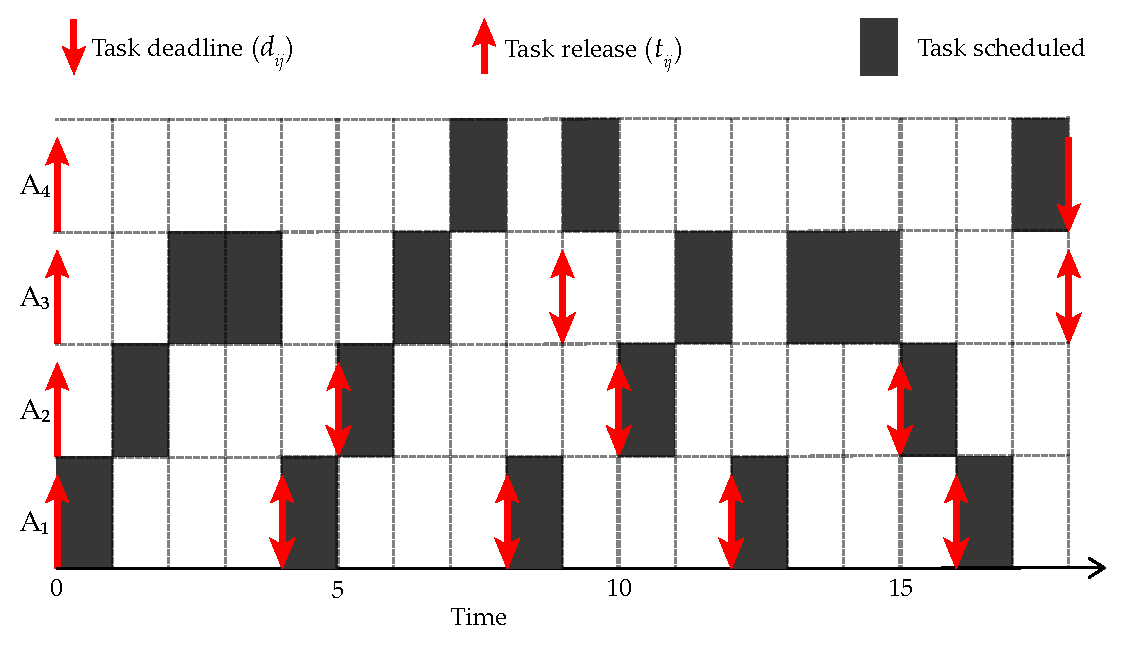
\includegraphics[width=\textwidth]{fpschedule}
    \caption[An example FPRM schedule.]{An example FPRM schedule using the task set from Table \ref{tab:example_task_set}.}
    \label{f:fp-schedule}
\end{figure}
\begin{figure}[t]
	\centering	
	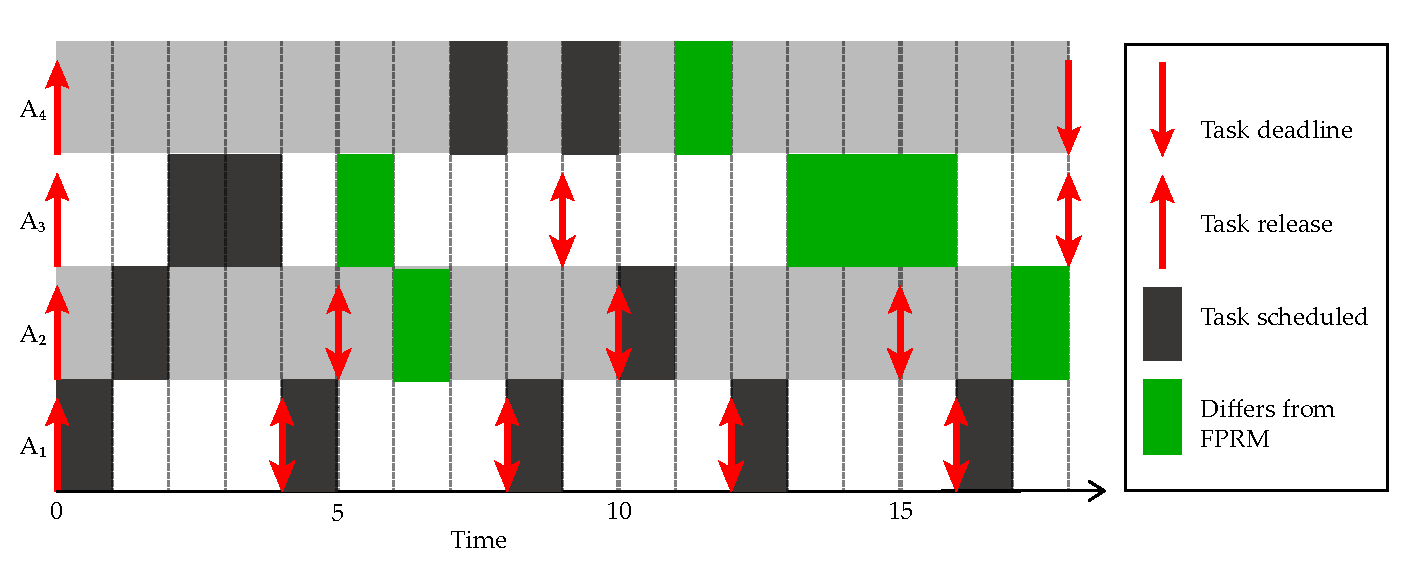
\includegraphics[width=\textwidth]{edfschedule}
    \caption[An example EDF schedule.]{An example EDF schedule using the task set from Table \ref{tab:example_task_set}.}
	\label{f:edf-schedule}
\end{figure}

\gls{EDF} is compatible with fixed-priority scheduling, as \gls{EDF} can be mapped to priority bands
in a fixed-priority system. Whenever an \gls{EDF} priority is selected, a second-level \gls{EDF}
scheduler dispatches the next task. This ``EDF in fixed-priority'' approach has been analysed in
detail~\citep{Harbour_Palencia_03} and is deployed in the Ada programming
language~\citep{Burns_Wellings:crtpa}, often used to build real-time systems.

\subsection{Earliest Deadline First versus Fixed Priority Scheduling}
\label{s:overload}
\TODO{Clarify what is and isn't a misconception: main one is overload, rest are BS}

\gls{EDF} is less popular in commercial practice than \gls{FP} for a number of reasons.  \gls{EDF}
is considered more complex to implement and to have higher overhead-related capacity loss.
Both algorithms have different behaviour under overload, and many consider the \gls{FP} behaviour
preferable.  Consequently, \gls{FP}
is mandated by the POSIX standard.

One common argument for
\gls{FPRM} is the idea that the algorithmic capacity loss is mediated by the overhead related
capacity loss of \gls{EDF}, and much easier to implement. 

However, all of these points were debunked by \citet{Buttazzo_05}.  Although \gls{EDF} is difficult
and inefficient to implement on top of existing, priority-based \glspl{OS}, both schedulers
can be considered equally complex to implement from scratch.  \gls{FP} scheduling has higher
overhead-related capacity loss due to an increase in the amount of preemption.  This compounds the
algorithmic capacity loss, rendering \gls{EDF} a clear winner in from-scratch implementations.

Other comparisons between \gls{EDF} and \gls{FP} are the complexity of their schedulability tests.
\gls{EDF} and \gls{FP} scheduling both have pseudo-polynomial
schedulability tests under the sporadic task model, although \gls{EDF} under the periodic task
model\footnote{The periodic task model is the same as the sporadic task model, with the restriction
that deadlines must be equal to periods ($d = p$), while periods themselves are considered absolute,
not minimum.} has an $O(n)$ schedulability test.  Like all pseudo-polynomial problems,
approximations can be made to reduce the complexity, although this comes with an error factor which
may not be suitable for \gls{HRT} systems.  

Both algorithms behave differently under constant
overload. \gls{EDF} allows progress for all jobs but at a lower rate, while \gls{FP} will
continue to meet deadlines for jobs with higher \gls{RM} priorities, completely starving other
jobs. Whether these behaviours are desirable is subject to context, under
transient overload conditions both algorithms can cause deadline misses.

% TODO mention reneging?

\subsection{Multiprocessors}

Both fixed and dynamic scheduling algorithms scheduling can be used on multiprocessor machines, either
\emph{globally} or \emph{partitioned}. Global schedulers share a single scheduling data structure
between all processors in the system, whereas partitioned schedulers have a scheduler per processor.
Neither is perfect: global approaches suffer from scalability issues such as hardware contention,
however partitioned schedulers require load balancing across cores.  Partitioning itself is known to
be a NP-hard bin-packing problem.  On modern hardware, partitioned schedulers outperform global
schedulers~\citep{Brandenburg:phd}.  For clustered multiprocessors a combination of global and
partitioned scheduling can be used; global within a cluster, and partitioned across clusters.

\section{Resource sharing}
\label{sec:resource-sharing-theory}

In the discussion so far we have assumed all real-time tasks are separate, and do not share resources.
Of course, any practical system involves shared resources. In this section we introduce the basics
of resource sharing, and the complexities of doing so in a real-time system.

Access to shared resources requires \emph{mutual exclusion}, where only one 
task is permitted to access a resource at a time, to prevent system corruption. Code that
must be accessed in a mutually exclusive fashion is called a \emph{critical section}. Generally
speaking, tasks lock access to resources, preventing other tasks from accessing that resource
until it is unlocked. However, many variants on locking protocols exist, including locks that permit
$n$ tasks to access a section, or locks that behave differently for read and write access.

Resource sharing in a real-time context is more complicated than standard resource sharing and
synchronisation, due to the problem of \emph{priority inversion}, which threatens the temporal
correctness of a system.  Priority inversion occurs when a low priority task prevents a high
priority task from running.  Consider the following example: if a low priority task locks a resource
that a high priority task requires, then the low priority task can cause the high priority task to
miss its deadline.  Consequently, all synchronised resource access in a real-time system must be
bounded, and the deadlines of tasks must account for those bounds.

Bounded critical sections alone are not sufficient to guarantee correctness in a real-time
system. Consider the scenario outlined earlier, where a low priority thread holds a lock that a high
priority thread is blocked on.  If other, medium-priority tasks exist in the system, then the low
priority task will never run and unlock the lock, leaving the high priority task blocked for an
unbounded period.  This exact scenario caused the Mars Pathfinder to fault, causing unexpected
system resets~\citep{Mars_Pathfinder}.

In this section we provide a brief overview of real-time synchronisation protocols that
avoid unbounded priority inversion, drawn from \citet{Sha_RL_90}. First we consider uniprocessor
protocols before canvassing multiprocessor resource sharing.

\subsection{Non-preemptive critical sections}

Using the \gls{NCP}, preemption is totally disabled whilst in a critical section.  This approach blocks
all threads in the system while any client accesses a critical section.  Consequently, the bound on
any single priority inversion is the length of the longest critical section in the system.  Although
functional, this approach results in a lot of unnecessary blocking of higher priority threads.  The
maximum bound on priority inversion that a task can experience is the sum of the length of all
critical sections accessed by that task, as these are the only places that specific task can be
blocked while other tasks run. 

\subsection{Priority Inheritance Protocol}
\label{sec:pip}

In the \gls{PIP}, when a high priority task encounters a locked resource, it donates its priority 
to the task holding the lock and when the lock is released the priority is restored. 
This approach avoids blocking any higher priority threads that do not access this resource, and
works for both fixed and dynamic priority scheduling.
However, \gls{PIP} results in a large preemption overhead and as a result has poor WCET analysis.

To understand this, consider a task set with $n$ tasks, $A_{1}, \ldots, A_{n}$, where each task's priority
corresponds to its index, such that the priority of $A_{i} = i$. The highest priority is $n$ and the
lowest is 1 and all tasks access the same resource. If $A_{1}$ holds the lock to that resource, then
the worst preemption overhead occurs if $A_{2}$ wakes up, elevating the priority of $A_{1}$ to 2. Subsequently,
each task wakes up in increasing priority order, each preempting $A_{1}$ until its priority reaches
$n$ resulting in $n$ total preemptions. 

Another disadvantage of \gls{PIP} is that deadlock can occur if resource ordering is not used.


\subsection{Immediate Priority Ceiling Protocol}
\label{sec:hlp}
\label{sec:ipcp}

Under \gls{IPCP}, also known as the highest lockers' protocol, resources are assigned a
\emph{ceiling} priority: the highest priority of all tasks that access that resource + 1.  When tasks
lock that resource, they run at the ceiling priority, removing the preemption overhead
of \gls{PIP}.

The disadvantage of \gls{IPCP} is that all priorities of task that access locked resources must be known \emph{a
priori}.  Additionally, if priority ceilings are all set to the highest priority, then behaviour
degrades to that of \gls{NCP}. Finally, this protocol allows intermediate priority tasks that do not need
the resource to be blocked. 

\subsection{Original Priority Ceiling Protocol}

The \gls{OPCP} combines the previous two approaches, and avoids deadlock, excessive blocking and
excessive preemption. In addition to considering the priorities of tasks, \gls{OPCP} introduces
a dynamic global state referred to as the \emph{system ceiling}, which is the highest
priority ceiling of any currently locked resource. When a task locks a resource, its priority 
is not changed until another task attempts to acquire that resource, at which point the resource
holder's priority is boosted to the resource's ceiling. By delaying the priority boost the excessive 
preemption of \gls{PIP} is avoided. Additionally, tasks can only lock resources
when their priority is higher than the system ceiling, otherwise they block until this condition is
true, thus avoiding the risk of deadlock. \gls{OPCP} results in less blocking overall than \gls{IPCP},
however requires global state to be tracked across all tasks, even those that do not share
resources, increasing the complexity of an implementation.

Neither protocol requiring resource ceilings is suitable for dynamic priority scheduling algorithms
like \gls{EDF}, however analogous algorithms exist, namely the \gls{SRP}~\citep{Baker_91}.

\subsection{Other locking protocols}

\TODO{Is there a reference for this subsection / I don't get why lock-free and wait-free can't be
used?}
We do not consider lock-free and wait-free algorithms in detail in this chapter, but note while
these may be deployed in real time systems there are always resources that need true blocking in
order to access them; in a word, stateful devices. For memory based resources, there is no need for 
algorithms that avoid blocking, as long as the total blocking time is bounded 
and fairness is not mandated. Any approach that is 
transactional with no guarantee of progress is not suitable, additionally, fair algorithms are not suited to a
real-time system, which are fundamentally not fair. 

\subsection{Summary}

\begin{figure}[ht]
  \centering
  \setlength{\unitlength}{1mm}
  \begin{picture}(50,25)(-5,-5)
    % WHOA! My first use of the picture environment in 25 years ;-)
    \thicklines
    \put(-5,0){\vector(1,0){50}}
    \put(7,-4){Priority inversion bound}
    \put(0,-5){\vector(0,1){25}}
    \put(-4.5,2){\rotatebox{90}{Complexity}}
    \put(2,15){OPCP}
    \put(12,3){IPCP}
    \put(25,11){PIP}
    \put(35,1.5){NCP}
  \end{picture}
  \caption[Comparison of RT locking protocols.]{Comparison of real-time locking protocols based on
    implementation complexity and priority inversion bound.}
  \label{f:locking}
\end{figure}

\Cref{f:locking} compares the different uniprocessor locking protocols, showing that \gls{OPCP}
provides the lowest bound on priority inversion; however is also the most complicated to implement.
\gls{NCP} on the other hand, is the simplest to implement but exhibits the worst priority inversion
behaviour, with \gls{PIP} and \gls{IPCP} falling between the two.  \gls{IPCP} provides minimal
implementation complexity but requires a policy on priority assignment to be in place in the system.

\subsection{Multiprocessor locking protocols}

Resource sharing on multiprocessors is far more complicated than the single processor case and still
a topic of active research. Of course, uniprocessor techniques can be used for resources that are
local to a processor, but further protocols are required for resources shared across cores (termed
\emph{global} resources).

Protocols for multiprocessor locking are either spinning- or suspension-based;
\emph{spinning} protocols spin on shared memory; \emph{suspension} protocols block the
task until the resource is available, such that other tasks can use the processor during that time.
Spin-lock protocols are effective for short critical sections, but once the critical section exceeds
the time taken to switch to another task and back, semaphore protocols are more efficient. 

Multiprocessor locking protocols differ depending on the scheduling policy across cores; in
partitioned approaches, priorities on different cores are not comparable, meaning existing protocols
do not work. While the protocols we have examined so far can be used under global scheduling,
\citet{Brandenburg:phd} showed that partitioned approaches suffer far less cache overheads than
global scheduling. 

The \gls{MPCP}~\citep{Rajkumar_90} is a modified version of \gls{OPCP} for multiprocessors. It is a
suspension-based protocol that works by boosting task priorities. Tasks run at the highest priority
of any task that may access a global resource, and waiting tasks block in a priority queue. Nested
access to global resources is disallowed. The \gls{MSRP}~\citep{Gai_DL_03} is a spin-lock based
protocol, which can be used for \gls{FP} and \gls{EDF} scheduling. \gls{MSRP} uses the \gls{SRP} locally,
combined with \gls{FIFO} spin-locks which guard global resources. 

Multiprocessor real-time locking protocols are an extensive field of research, and 
many more sophisticated locking protocols exist, however we do not survey them here.

\section{Operating systems}
\label{sec:background-operating-systems}

An \gls{OS} is a software system that interfaces with hardware and devices in order to present a
common interface to applications.  The \emph{kernel} is the part of the operating system that
operates with privileged access to the processor(s) in order to safely perform tasks that allow
applications to run independently of each other.

Common \glspl{OS}, such as Windows, MacOS and Linux, are \emph{monolithic} operating systems,
which means that many services required to run applications are inside the kernel.  A \emph{microkernel}
attempts to minimise the amount of code running in the kernel in order to reduce the amount of
trusted code.  Figure \ref{fig:os-microkernel} illustrates the difference between monolithic
\glspl{OS} and microkernels.  Modern microkernel implementation is guided by the minimality
principle~\citep{Liedtke_95} which aims to provide minimal mechanisms to allow resource servers to
function, leaving the rest of the policy up to the software running outside of the kernel. According
to the minimality principle, if a service does not need to be in the kernel to achieve its
functionality, it should not be in the kernel.

\begin{figure}[tb]
	\begin{center}
		\leavevmode
		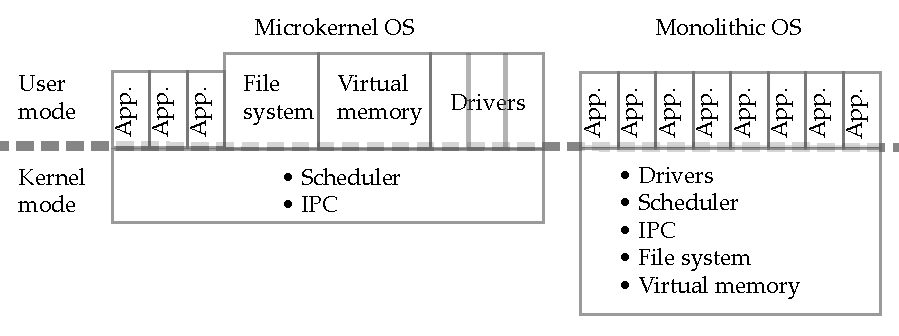
\includegraphics{os-microkernel.pdf}
		\caption{Structure of a microkernel versus monolithic operating system.}
		\label{fig:os-microkernel}
	\end{center}
\end{figure}

Monolithic operating systems provide scheduling, \gls{IPC}, device drivers, memory allocation, file
systems and other services in the kernel, resulting in a large \emph{trusted computing base}.

With respect to microkernels, interpretations of the minimality principle varies, 
consequently which services and utilities are included in the privileged kernel varies. In
larger kernels thread scheduling, memory allocation and some device drivers are included in the kernel.
For example, \selfour~\citep{Klein_EHACDEEKNSTW_09} contains scheduling and \gls{IPC}; 
\composite~\citep{Parmer:phd} does not provide a scheduler, or any blocking semantics, but does
provide \gls{IPC}. 

Microkernels are far more amenable for deployment in areas where security is a primary concern,
due to their small trusted computing base.
Services on top of the microkernel can be isolated and assigned different levels of trust, unlike
the services in a monolithic \gls{OS} which all run at the same privilege level such that a fault in
one service can compromise the entire system. 

Operating systems can run on each other in a process called \emph{virtualisation}, where the
underlying OS presents an interface imitating hardware. A \emph{hypervisor} is an operating system that can
run other operating systems on top of it, and operating systems running on the hypervisor are
referred to as \emph{guests}. Guest operating systems can be para- or fully-virtualised, where the
former involves modifications to the source of the guest. Modern hardware has virtualisation
extensions which improve virtualisation performance and reduce the need for para-virtualisation.
Both microkernels and monolithic kernels can also be hypervisors, although monolithic hypervisors
are often smaller than full OS counterparts, as they provide less functionality and rely on guest
OSes to provide most systems. 

\subsection{Capabilities}
\label{s:b-capabilities}

Many security-focused microkernels make use of \emph{capabilities}~\citep{Dennis_VanHorn_66}, an
established mechanism for fine-grained access control to spatial resources which allow for spatial
    isolation. A capability is a unique, unforgeable token that gives the possessor permission to access
an entity or object in system. Capabilities can have different levels of access rights, e.g. read,
write, execute etc. 

By combining access rights with object identifiers capabilities avoid the
confused deputy problem, a form of privilege escalation where a deputy program
acting on behalf of a client is  tricked into using
its own rights to manipulate a resource that the client would not normally have access
to~\citep{Hardy_88}. 

\subsection{IPC}
\label{s:background-ipc}

\gls{IPC} is the microkernel mechanism for synchronous transmission of data and capabilities between
processes. Because the microkernel model provides services encapsulated into user-level servers,
\gls{IPC} is key to microkernel performance, as it is used more predominantly than in monolithic
\glspl{OS}. Originally, microkernels were criticised as impractical due to inefficient IPC
implementations of first-generation microkernels. However, this was demonstrated to be
false~\citep{Hartig_HLSW_97} due to the high cache footprint and poor design of the original
microkernels. Second-generation microkernels were built much leaner, with fewer services in the
kernel and fast, optimised code paths for IPC, referred to as \emph{fastpaths}. 
\emph{Third-generation} microkernels follow the pattern of minimality and speed, whilst also
promoting security as a first-class concern, which resulted in the incorporation of capability
systems. 

\subsection{Open vs. Closed Systems}

Operating systems can be built for open or closed systems.  An \emph{open system} is any system
where code outside of the control of the system designers can be executed. For example, modern
smart phones are open systems, given that users can install third-party applications.

A \emph{closed system} is the opposite; the system designers have complete control over all code
that will execute on the system.  The majority of closed systems are embedded, including those found
in cars, spacecraft and aircraft.

In general, there is a trend toward systems becoming more open; initial mobile phones were closed
systems.  This trend can be perceived from infotainment units in automobiles to televisions, where
the option to install third party applications is becoming more prevalent.  Allowing third-party
applications to run alongside critical applications on shared hardware increases the security
requirements of the system: critical applications must be isolated from third-party applications and
secure communications must be used between distributed components.  This is currently not the
general case, which has led to researchers demonstrating attacks on
cars~\citep{Checkoway_MKASSKCRK_11}.

Open systems are generally \emph{dynamic}---where resource allocations are configured at run-time
and can change---as opposed to closed systems which have \emph{fixed} or \emph{static} resource
allocation patterns.

%% introduce RTOSes
\subsection{Real-Time Operating Systems}

A \gls{RTOS} is an \gls{OS} that provides temporal guarantees, and can be microkernel-based or
monolithic.  Whilst some real-time systems run without operating systems at all, this approach is
generally limited to small, closed systems and is both inflexible and difficult to
maintain~\citep{Lui_AACBBBCLM_04}.

In a general purpose \gls{OS}, time is shared between applications with the aim of providing
\emph{fairness}, where applications share the processor equally.  This fairness is not divided into
equal share, but weighted, such that some applications are awarded more time than others in order
to tune overall system performance.  The \gls{OS} itself is not directly aware of the timing needs of
applications.

In an \gls{RTOS}, fairness is replaced by the need to meet deadlines. As a result, time is promoted
to a first class resource~\citep{Stankovic_88}.

Time being an integral part of the system affects every other part of the \gls{OS}.  For example, in
an \gls{RTOS}, one application having exclusive access to a resource cannot be allowed to cause a
deadline miss.  Similarly, the \gls{RTOS} itself cannot cause a deadline miss.  This means that all
operations in the \gls{RTOS} must either be bounded with known {\gls{WCET}} or the \gls{RTOS} must
be fully preemptible.  However, it must be noted that a fully preemptible \gls{OS} is completely
non-deterministic, making correctness impractical to guarantee~\citep{Blackham_TH_12}.  The overheads
of \gls{RTOS} operations like interrupt handling and context switching must also be considered when
determining whether deadlines can be met.

Traditional \glspl{RTOS}, and the applications running on them, require extensive offline analysis
to guarantee that all temporal requirements are met.  This is done by using scheduling algorithms,
\gls{WCET} analysis, and resource sharing algorithms with known real-time properties.

\subsection{Resource kernels}
\label{sec:resource-kernels}

Resource kernels are a class of \gls{OS} that treat time as a first class resource, by providing
timely, guaranteed access to system resources.  In a resource kernel, a reservation represents a
portion of a shared resource, like processor, or disk bandwidth.  Unlike traditional real-time
operating systems, resource kernels do not trust all applications to stay within their specified
resource bounds: resource kernels enforce them, preventing misbehaving applications from interfering
with other applications and thus providing temporal isolation.

In the seminal resource kernel paper, \citet{Rajkumar_JMO_98} outline four main goals that are
integral to resource kernels:
\begin{description}
    \item[G1: Timeliness of resource usage] Applications must be able to specify resource
        requirements that the kernel will guarantee.  Requirements should be dynamic: applications
        must be able to change them at run-time, however the kernel should ensure that the set of
        all requirements can be admitted.
    \item[G2: Efficient resource utilisation] The mechanisms used by the resource kernel utilise
        available resources efficiently and must not impose high utilisation penalties.
    \item[G3: Enforcement and protection] The kernel must enforce resource access such that rogue
        applications cannot interrupt the resource use of other applications.
    \item[G4: Access to multiple resource types] The kernel must provide access to multiple resource
        types, including processing cycles, disk bandwidth, network bandwidth and virtual memory.
\end{description}

In another paper, \citet{deNiz_LSR_01} outline the four main mechanisms that a resource kernel must
provide, in order to implement the above concepts.

\begin{description}
	\item[Admission] check that all resource requests can be scheduled (\textbf{G1}).
	\item[Scheduling] implements the dynamic allocation of resources according to reservations (\textbf{G1, G2}).
	\item[Enforcement] limit the consumption of the resources to that specified by the
        reservation (\textbf{G3}).
	\item[Accounting] of reservation use, to implement scheduling and enforcement (\textbf{G1, G2, G3}).
\end{description}

\label{p:resource-kernel-resource-sharing}
In order to share resources in a resource kernel, avoiding priority inversion becomes a more
complicated problem.  \citet{deNiz_LSR_01} outline three key policies that must be considered when
handling resource sharing in reservation-based systems:

\begin{description}
    \item[Prioritisation] What (relative) priority is used by the task accessing the shared resource (and under what conditions)?
    \item[Charging] Which reservation(s), if any, gets charged, and when?
    \item[Enforcement] What happens when the reservations being charged by the charging policy expire?
\end{description}

Resource kernels are a form of monolithic operating system, where all system services and drivers
are provided by the kernel.  In a microkernel, not all the mechanisms of a resource kernel are
suitable for inclusion in the kernel itself: some can be provided by user-level middle-ware.  This
is because core resource kernel concepts contain both policy and mechanism.  We argue that the
microkernel should provide resource kernel mechanisms such that a resource kernel can be built with
a microkernel, but policy should be left up to the system designer, as long as it does not result in
performance or security concessions.

\section{Summary}

In this chapter we have briefly covered the core real-time theory that this thesis draws upon.
We have defined operating systems, and introduced the concepts that inform the design of resource kernels.
In the next chapter we will survey how these can be combined to achieve isolation and asymmetric protection for mixed-criticality systems.
